\documentclass[12pt]{article}
\usepackage{graphicx}
%% \usepackage{lineno}
%% \linenumbers

\title{Modeling transient mortality shocks in low-mortality populations}
\author{Joshua R. Goldstein \and Ronald D. Lee \\ Proposal for
  Presentation at PAA 2021 \\ Extended Abstract}

\begin{document}

\maketitle
\begin{abstract}

  The standard Lee-Carter model is useful for looking at the long-term
  evolution of progress in longevity but does not include the effect
  of short-term, transient shocks such as the life expectancy declines
  seen in recent years in the United States or the coronavirus
  epidemic.  In this work, we extend the Lee-Carter approach by adding
  an annual transitory component, meant to represent effects such as
  weather, economic shocks, and infectious diseases. Our preliminary
  findings show that the extended model works well for some, but not
  all, countries. The transient shocks we detect are correlated across
  countries, suggesting that they are picking up real external shocks
  to mortality, rather than measurement error. Our hope is that these
  models will be of use to understanding the magnitude and nature of
  modern mortality shocks, the implications of these shocks for
  future mortality trends, and the uncertainty in mortality forecasts.
  
  
\end{abstract}

\section{Overview}


The canonical time-series model used for studying modern mortality
trends is the Lee-Carter model with a random walk with drift. The
logic behind this is that there is a steady march of progress toward
lower mortality which varies in its pace. The recent three-year run of
declining life expectancy in the United States, the French heatwave of 2003,
the annual flu, and -- of course - the current coronavirus pandemic 
are all examples of transient shocks, highlighting that factors other
than technological progress and changes in population health
may be important for mortality in any given year.

Modeling these short-term transient shocks is interesting in its own
right, because of what it reveals about the nature of population
mortality levels and changes.  It may also be useful for understanding
the long-run implications of mortality reversals like that from the
U.S. opioid crisis or the worldwide coronavirus pandemic. A fuller
description of variation may also improve the estimation of
probability intervals for Lee-Carter type mortality forecasts by
ditinguishing long term and short term uncertainty, which the simple
random walk model does not and cannot do.

Here we present a model and preliminary results for the modeling of
transient mortality shocks, extending Lee-Carter estimates of the
evolution of mortality over time. The model we fit includes two random
terms: the first is the standard term for the evolution of the
underlying trend in the Lee-Carter model, a random walk with
deterministic drift; the second is a new term for transient shocks,
which we interpret as events due to weather, economic shocks, or
infectious disease outbreaks.

These preliminary models only work well for some
countries. Nonetheless it is still possible to see that the transient
shocks of neighbors are correlated, suggesting that they are picking
up real shocks to mortality, perhaps caused by the effects of severe
weather and contagious diseases.


\section{Modeling}

The approach we use to model mortality shocks is based on structural
time series approaches for distinguishing between long-lasting changes
from transient shocks. These models include two kinds of random terms,
one which influences the underlying state of the system and an
additional term that translates the state of the system into what is
observed at a given time. In our application, we think of mortality
rates as consisting of an underlying level of technology and
population health that evolves slowly over time, combining with
short-term fluctuations in conditions such as the weather and
contagious disease that can vary greatly from one year to the next.
Each year's observed mortality is the result of both factors. The
model tries to separate them.\footnote{Longer lasting but still
  transitory influences on mortality such as the HIV or opioid
  epidemics in the US, or life expectancy reversals after the fall of
  the Soviet Union, are in a grey area between the two, which the
  model will fit as best it can by combining these them. However, we
  hope to consider this case by further extending our model to include
  time-series structure in the $n(t)$ term presented below.}

We begin by using the standard Lee-Carter approach. This model reduces
the logarithm of the full set of age-period mortality rates to an
average age-schedule $a_x$ and a time index $k_t$ that drives
age-specific changes $b_x$. The model has the form
$$
\log M_{x,t} = a_x + b_x k_t.
$$

The usual time series model for forecasting used by Lee and Carter is
the random walk with drift
$$
k_t = k_{t-1} + d + \epsilon_t.
$$
To this, we add another layer to the estimation of the time series,
decomposing the observed $k_t$ into a latent $k_t$ that still evolves as a
random walk with drift as well as an annual transitory component $n_t$. In
state-space modeling $n_t$ is sometimes called ``observation
error'' or ``noise''. We are conceiving of it not so much as error but as a
transitory perturbation -- for example due to weather or the severity
of the annual flu or to another kind of contagious disease such as
COVID-19.

The model has the form

\begin{equation}
  k_t^{observed} = k_t^{latent} + n_t
\end{equation}

\begin{equation}
  k_t^{latent} = k_{t-1}^{latent} + d + \epsilon_t
\end{equation}

The model has two features.
\begin{itemize}
\item The observed value is the latent value plus ``noise'' $n_t$,
  which is assumed to be normally distributed with constant variance
  and independent over $t$ from one year to the next..

  \item The latent value evolves as a random walk with drift, with a
    fixed (deterministic) value of $d$.
\end{itemize}

(Note it is also possible to add an additional random layer to this
model by making $d$ itself a stochastic evolving term. The standard
form of this ``random trend'' model is to let $d$ evolve as a random
walk, $d_t = d_{t-1} + \eta_{t-1}$.  Other extensions include
considering non-normal distributions for $n_t$ as well as adding
time-series dependence to the evolution of $n_t$ over time. We don't
consider these extensions here.)

\section{Data and methods}

Because we are interested in short-term fluctuations that are often
small in magnitude, we limit our application to high-quality
data available in the Human Mortality Database. It would also be of
interest to include a broader range of countries, but this would
require a careful evaluation of data quality.

We estimate the Lee-Carter model using the {\tt demography} package
written by Hyndman et al. We model both sexes together and use the
option of calibrating the estimates of observed $k_t$ to life
expectancy at birth.

We estimate the structural time series models using the MARSS
(Multivariate Autoregressive State-Space Modeling)  package
written by by Holmes et al. 

We note that it is also possible to estimate short term shocks by
smoothing the observed time series and looking at differences between
the observed and smoothed rates. This produces similar results when we
look at the correlations between countries. An advantage of the time
series approach is that it it makes explicit the underlying
assumptions and nature of the model. A further advantage is that the
explicit time series model used to fit the past can also be used for
forecasting the future.


\section{Results}

We begin by showing the estimates of the latent $k_t$ for France in
Figure \ref{france_fig}. The time trend is generally downward, corresponding to
improvements in mortality rates over time. As expected the latent
$k_t$ is considerably smoother than the observed term. The
differences between observed and latent mortality correspond in some
cases to known shocks, such as the heat-wave of 2003 and the
global influenza (H3N2) of 1968.


\begin{figure}
  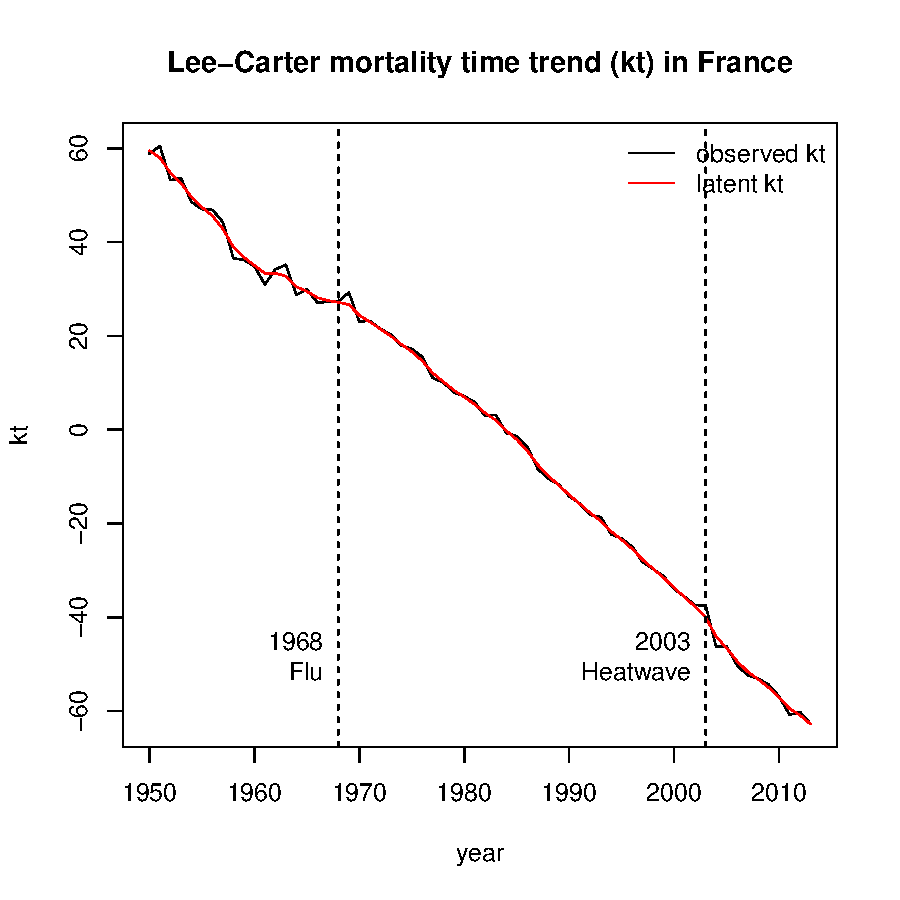
\includegraphics[width=1.05\textwidth]{../code/france_example.pdf}
  \caption{Estimates of observed and latent values of $k_t$ in
    Lee-Carter model using MARSS package based on HMD data. Mortality
    shocks for 1968 Flu (which reportedly had more severe death rates
    in Europe in 1969) and the 2003 heatwave are indicated.}
    \label{france_fig}
\end{figure}


Figure \ref{kt_panel_fig} shows the observed and latent $k_t$ for a larger set of
19 countries. Some cases resemble France in that one can clearly see that
the latent $k_t$ is a smoothed version of what is observed. However,
in other cases, such as the United States and Russia, the estimates of
the latent $k_t$ are so similar to what is observed as to make the two
lines essentially indistinguishable.

\begin{figure}
  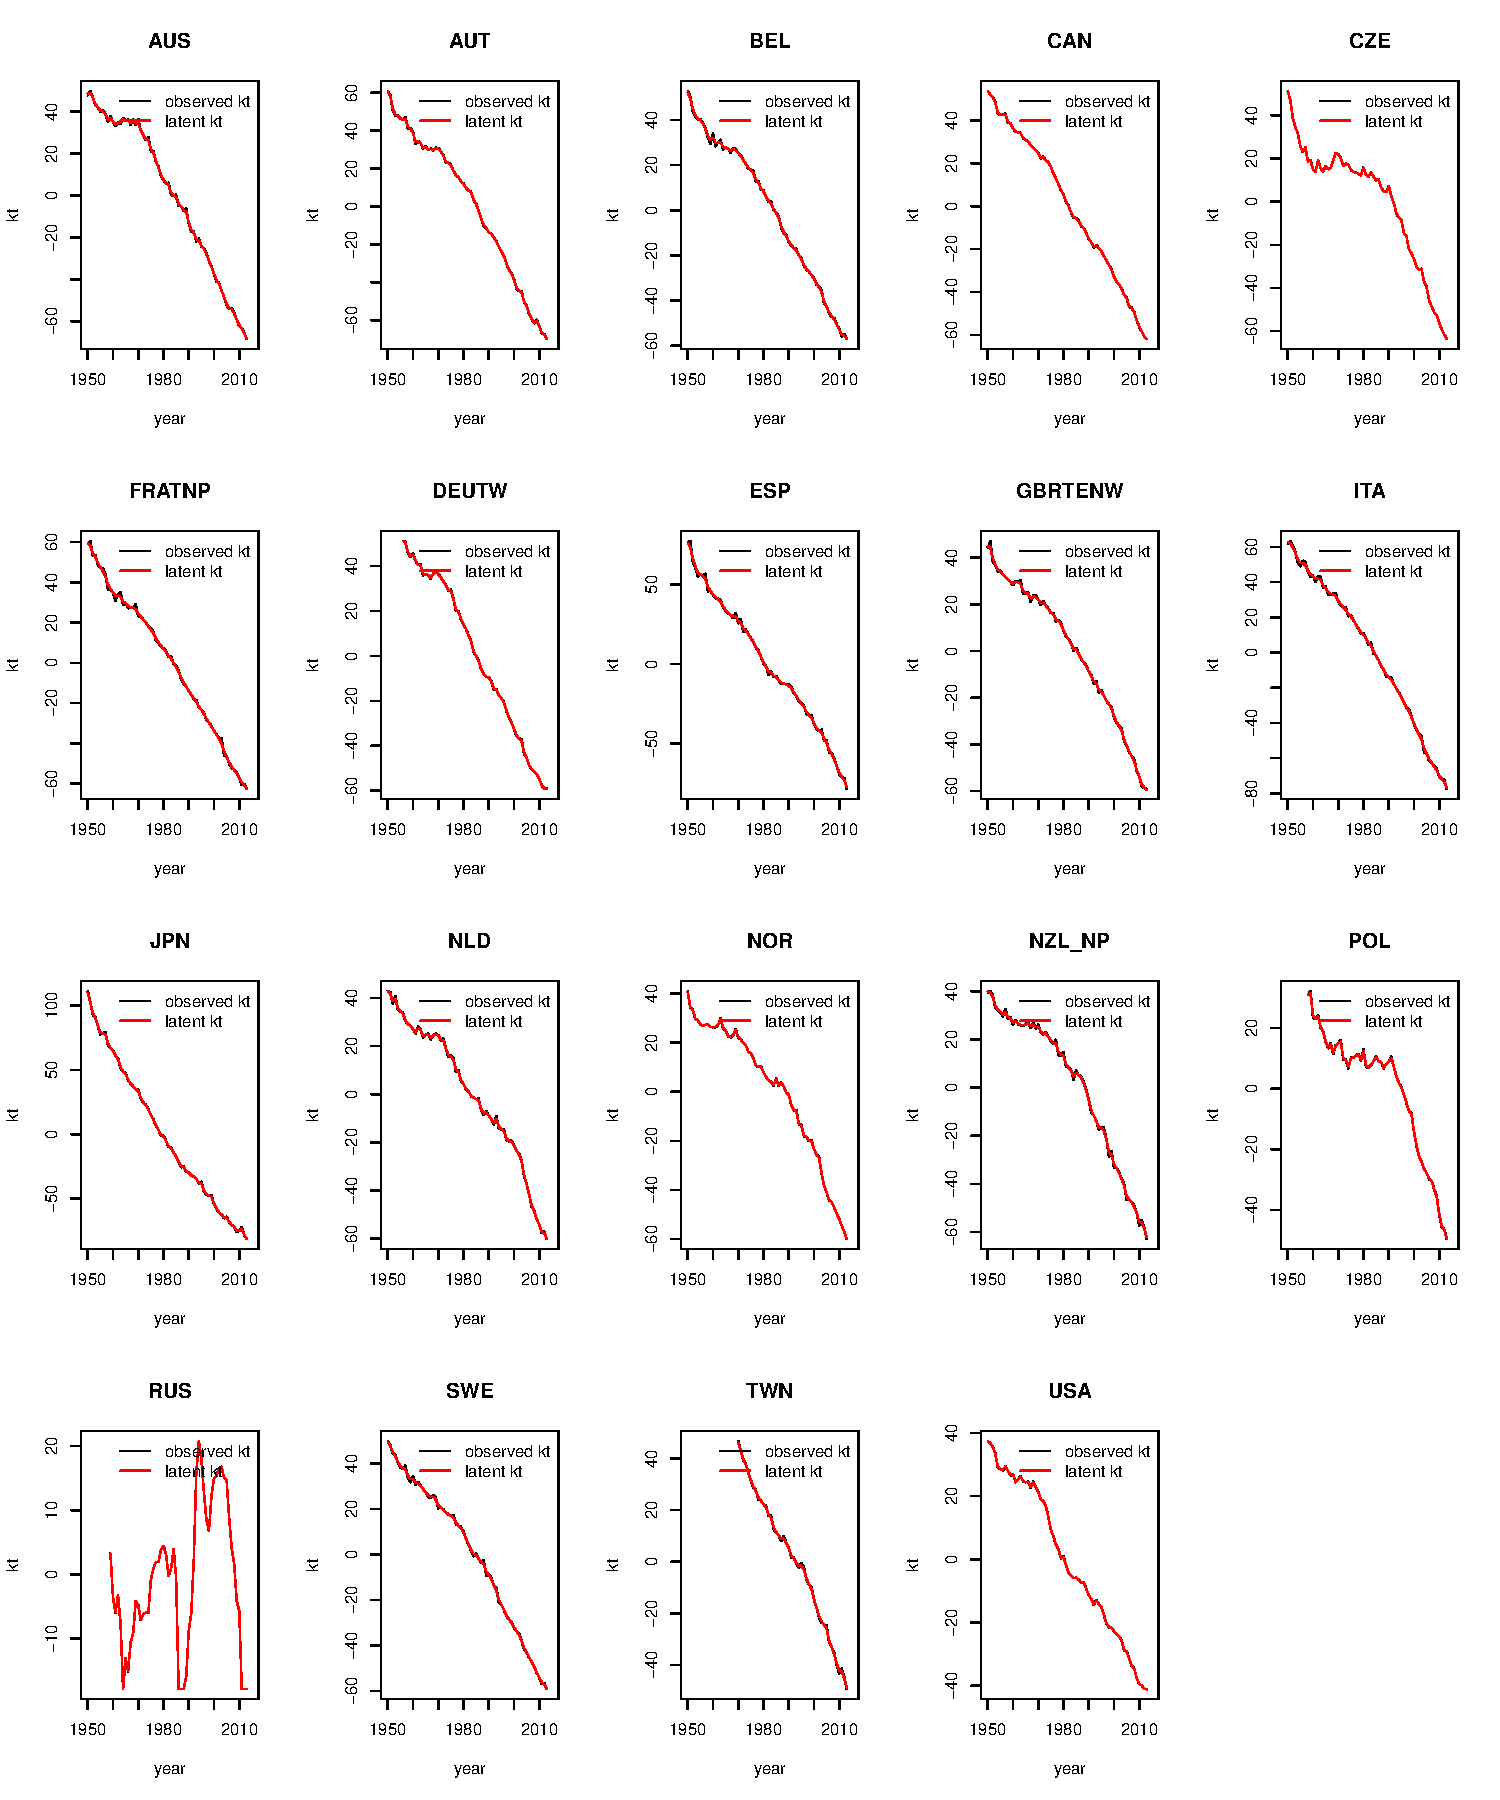
\includegraphics[width=1.05\textwidth]{../code/kt_panel_plot.pdf}
  \caption{Estimates of observed and latent values of $k_t$ in
    Lee-Carter model using MARSS package based on HMD data. Note: in
    some countries (e.g., Russian and the United States) the estimated
    shocks are so small that the latent and observed $k_t$ values are
    overlapping and indistuishable to the eye. }
    \label{kt_panel_fig}
\end{figure}


Figure \ref{nt_panel_fig} shows the same information as figure 2 in the form of the
differences between the observed and latent mortality time trends
($k_t$). These are plotted on the same scale to make it apparent that
the magnitude of the estimated transient shocks are similar in many
countries, including France, Sweden, Japan, Italy, Great Britain and
Spain, but smaller in West Germany, and even smaller in the United
States and Russia.

\begin{figure}
  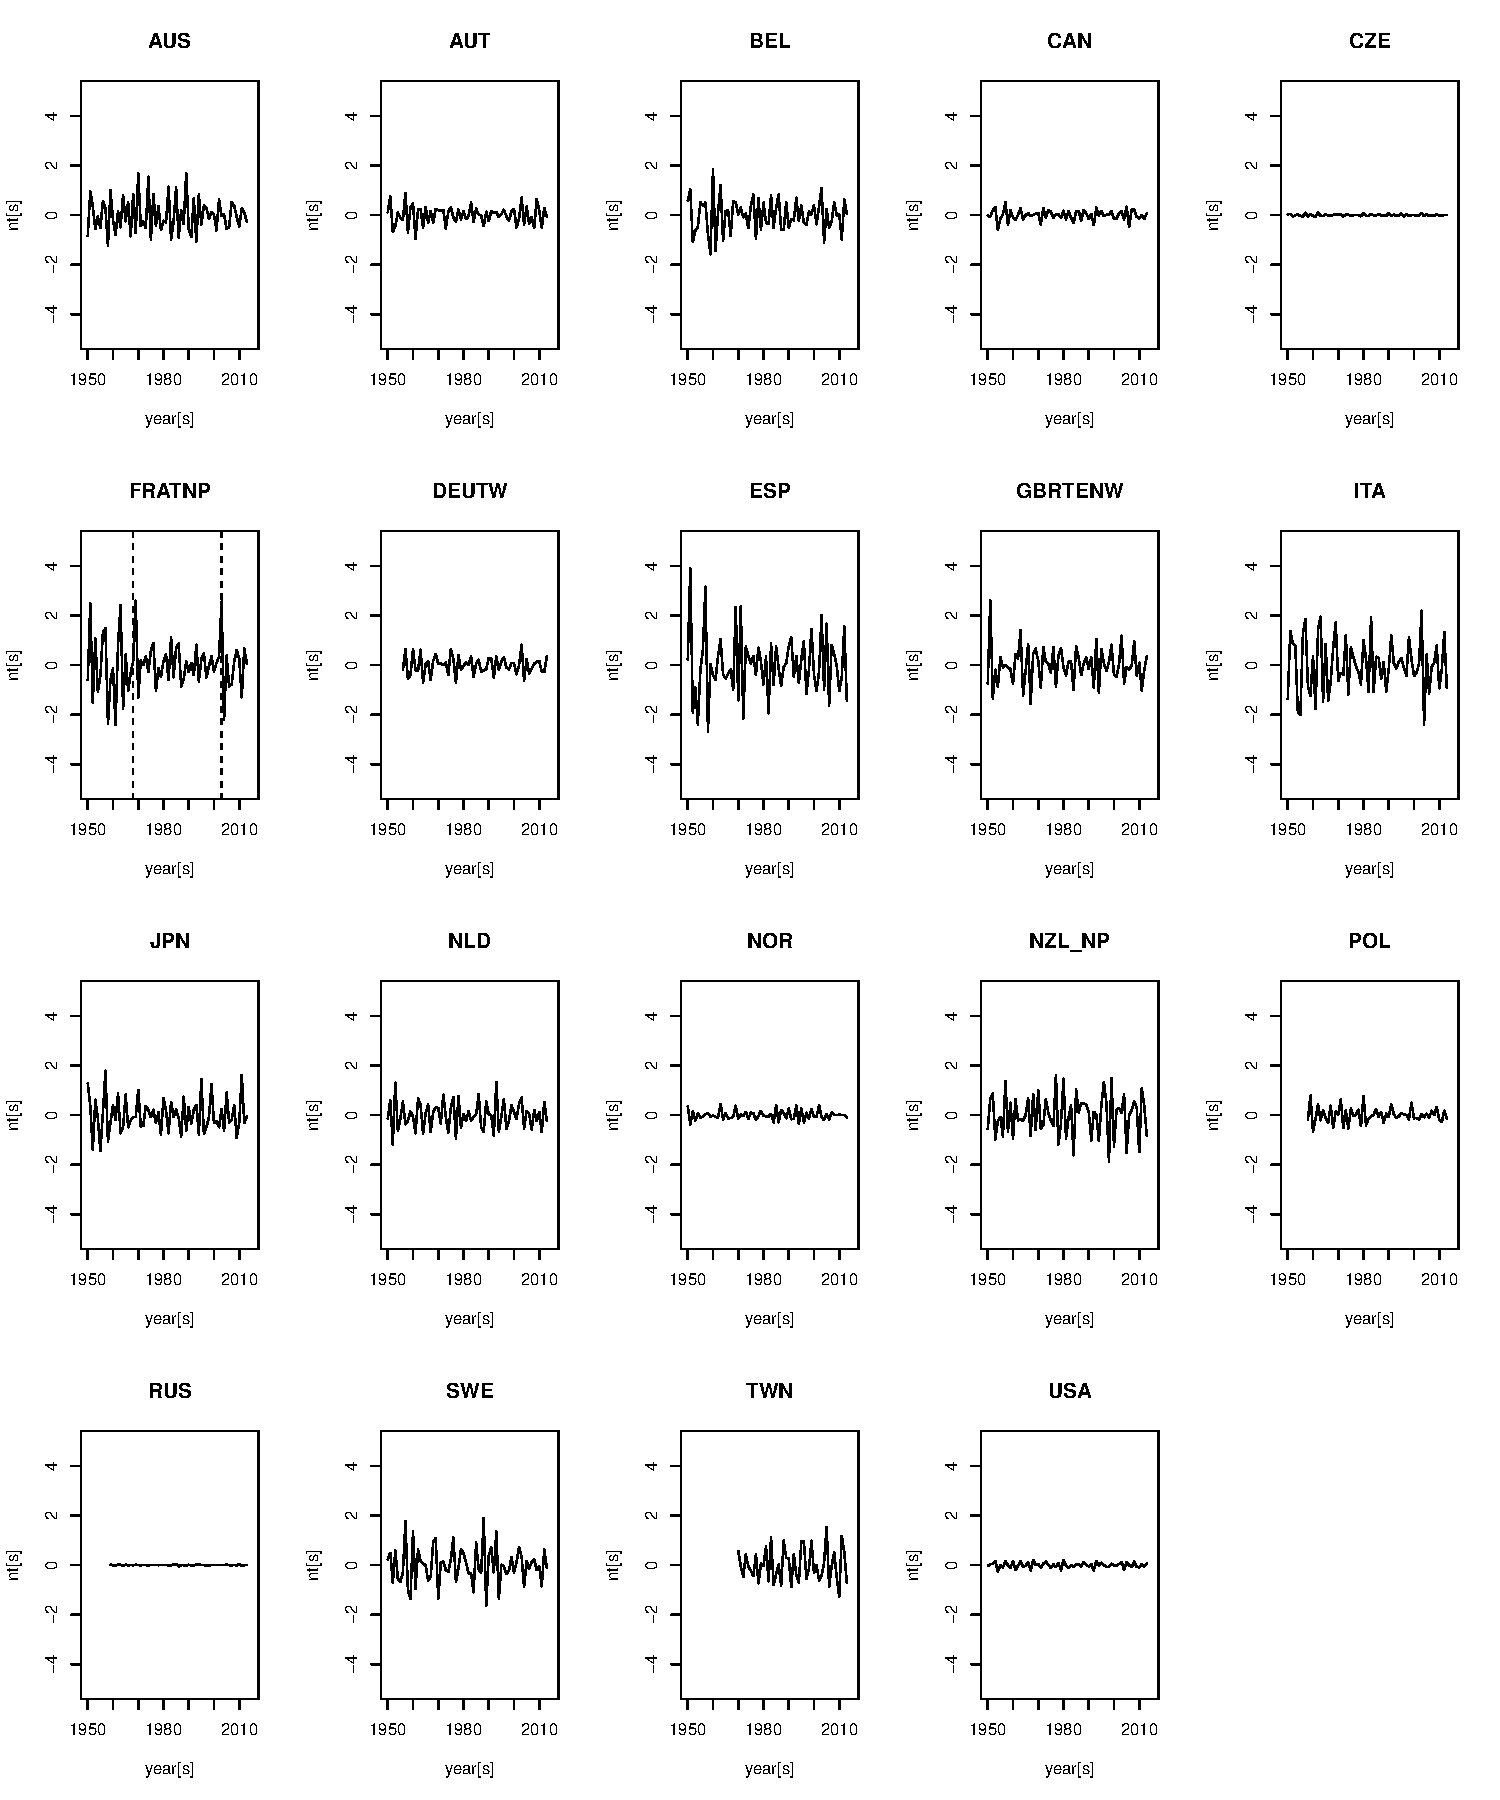
\includegraphics[width=1.05\textwidth]{./../code/nt_panel_plot.pdf}
  \caption{Estimated shocks $n_t = k_t^{latent} - k_t^{observed}$,
    shown on a common scale. Note: the vertical lines in the
    ``FRATNP'' panel correspond to the 1968 Flu and 2003 Heatwave
    shown in Figure \ref{france_fig}}
    \label{nt_panel_fig}
\end{figure}


One reason for the small magnitudes of mortality shocks estimates for
the United States and Russia is that the variations that we see in
these countries in the observed $k_t$ tend to consist less of high
frequency, year-to-year fluctuations and more of what appears to be
multi-year departures from trend. The estimation approach we are using
then assigns these departures from trend to persistent changes in the
latent state ($\epsilon_t$), rather than to a high-frequency transient effect.

This may be an undesirable idiosyncracy of the model we are using. On
the other hand, it may reflect something fundamentally different about
the evolution of mortality in some countries. The United States is a
large country consisting of many sub-populations and that may be part of
the reason it appears to evolve differently over time. The evolution
of mortality in Russia of course has been one of repeated crises in
recent decades and it is not surprising that the same time series
model that works well for France and Sweden behaves differently for
Russia.

Setting the magnitudes of the shocks aside, we can see if the timing
coincides across some countries, and if so, which countries experience
the same shocks at the same time.  In Figure \ref{nt_corr_fig}, we plot the shocks for
all pairs of countries and give the correlation, ordering them using
the 1st principle component. We see that the Continental European
countries (France, Germany, Blegium, Italy, Spain and Austria) appear
to be highly correlated. The English speaking countries (U.S, U.K, and
Canada) also have similar temporal patterns of mortality shocks. 

\begin{figure}
  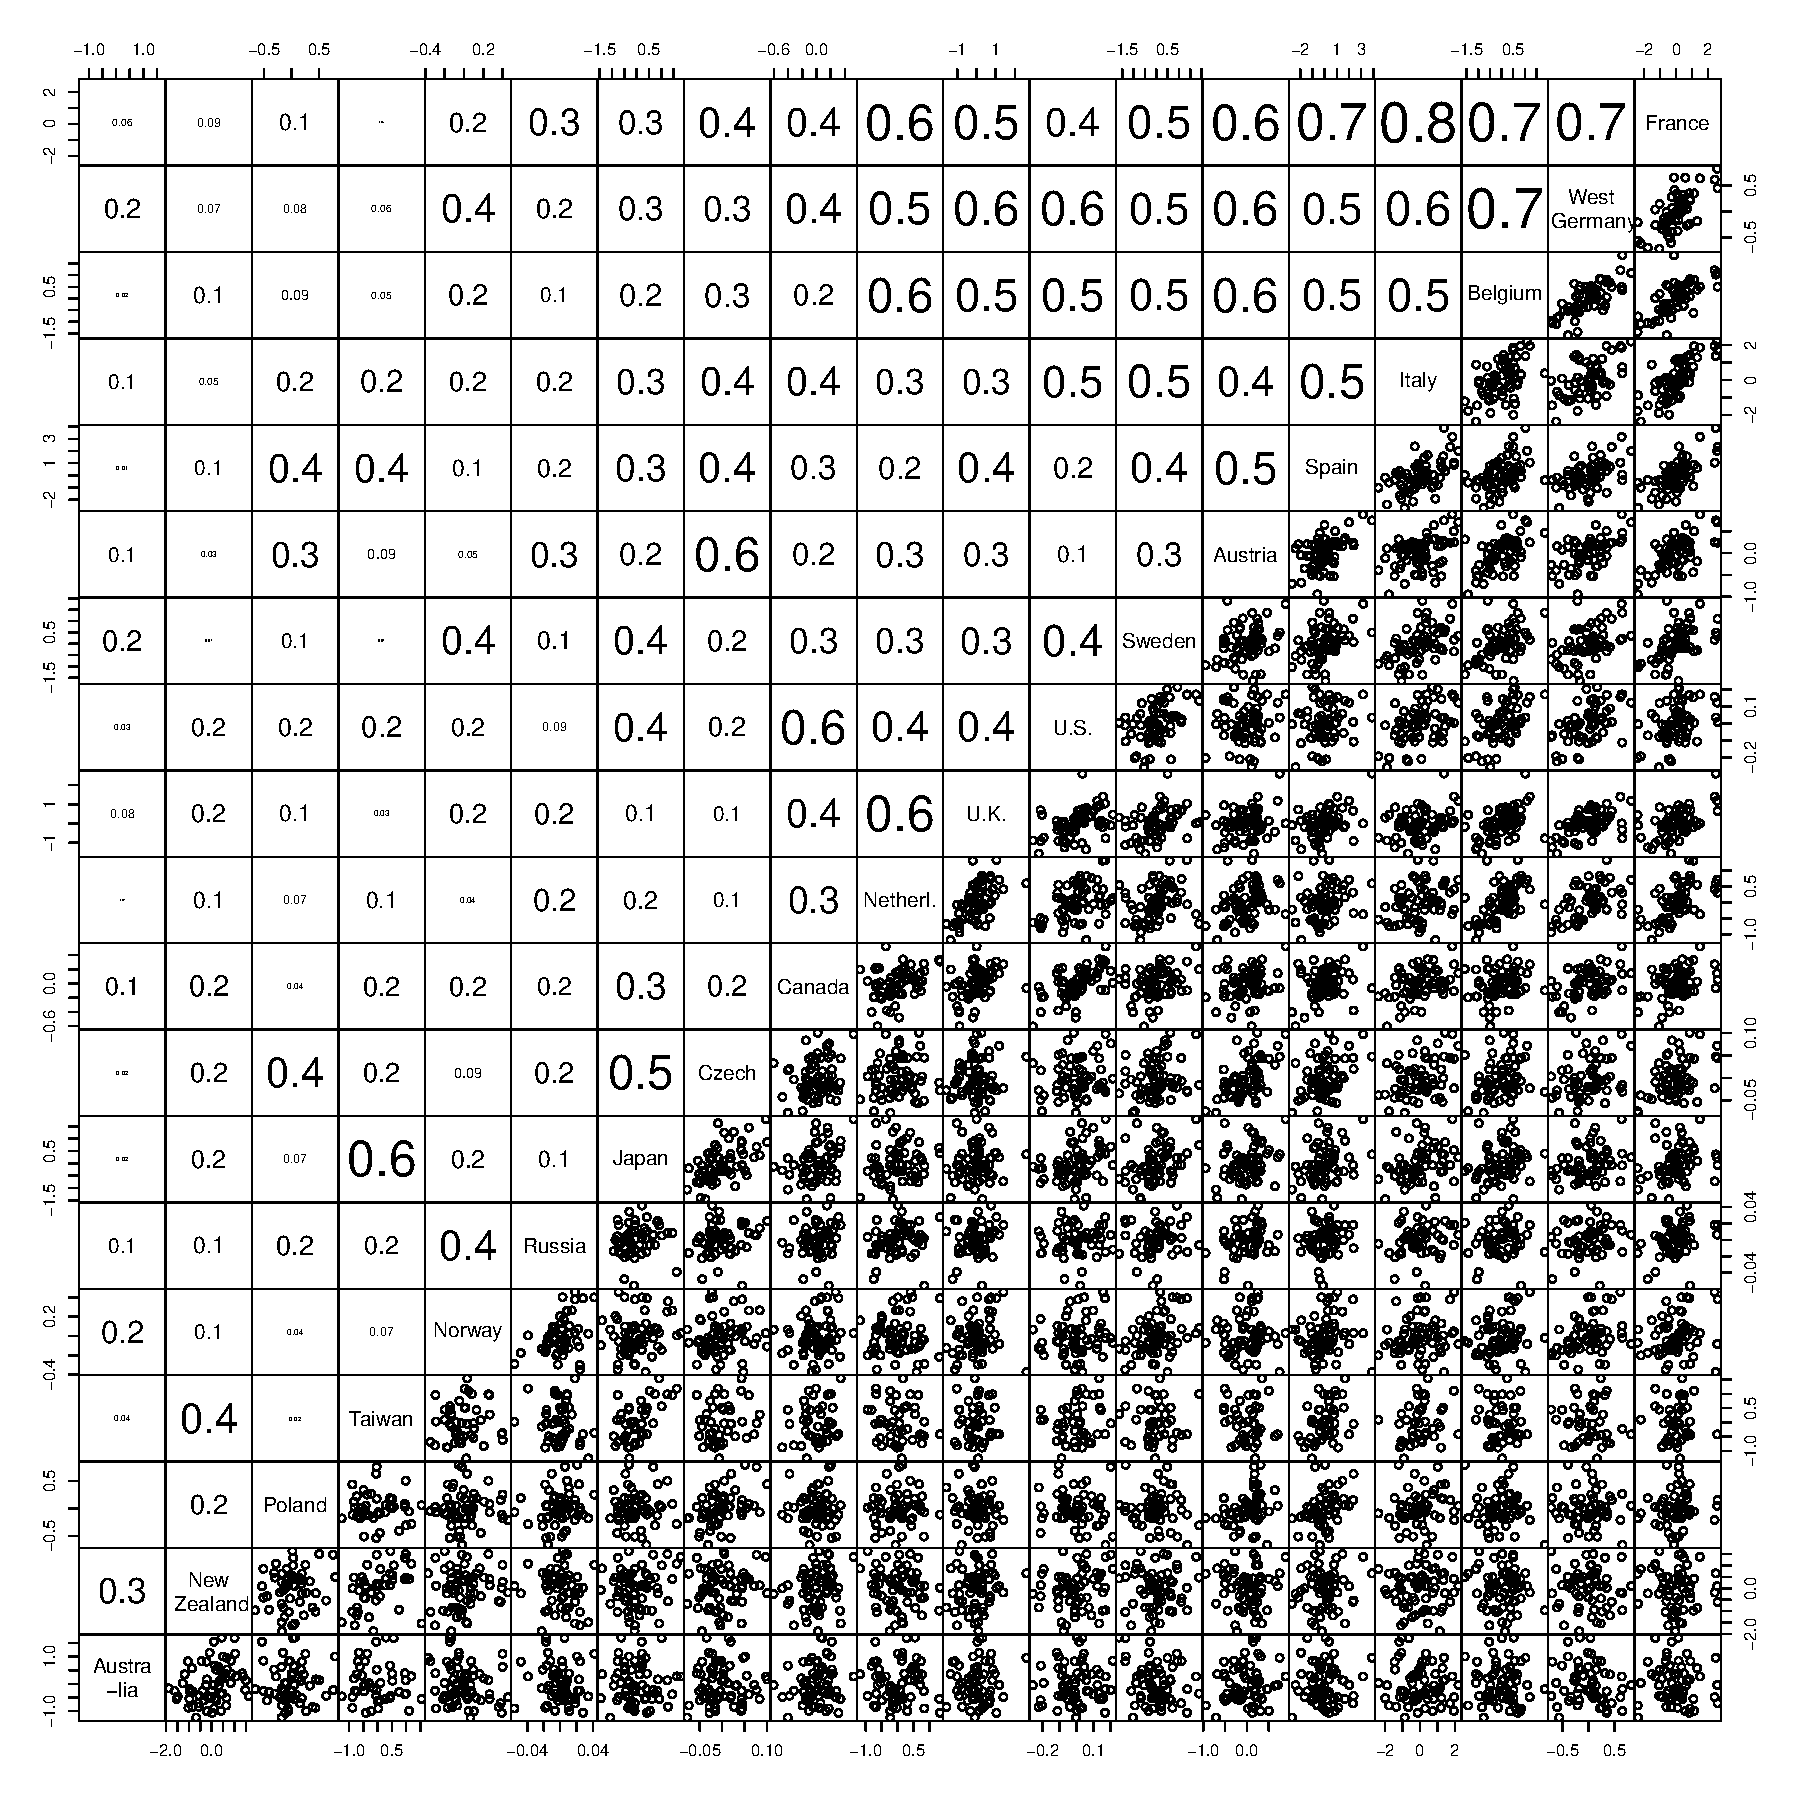
\includegraphics[width=1.05\textwidth]{./../code/nt_corr_plot.pdf}
  \caption{Bivariate scatter plots in annual short-term mortality
    shocks ($n_t$) among countries along with the corresponding
    correlation. The countries are ordered by the strength of
    correlation, as measured by the 1st principle component.  For
    example, the correlation between shocks measured in Canada and
    the United States is 0.6}
    \label{nt_corr_fig}
\end{figure}

The two countries with the highest correlation (0.8) in short-term
shocks are Italy and France. Other notable correlations include Taiwan
and Japan (0.6) and Austria and Czechoslovakia (0.6). Australia has
shocks that are largely uncorrelated with the rest of the world,
except New Zealand (0.3), and New Zealand is most correlated wtih
Taiwan (0.4).

There is some suggestive evidence that there is more than geographic
distance linking the short-term fluctuations in mortality. For
example, New Zealand is  more correlated with Canada, the United
States, and the U.K. than it is with continental European countries.
Some surprising correlations, e.g., between Japan and Czechoslakia
suggest that there may be some random element, too, in the
correlations we find and caution against over-interpretation. It may
be interesting to compare the correlation structure we find with trade
or travel patterns. 


\section{Discussion}

Our estimation of transitory mortality is not complete. But a few
preliminary conclusions can be reached.

\begin{enumerate}

\item The structured time series model of annual transient shocks
  appears to be a good description of what is happening in countries
  with otherwise steadily declining mortlaity such as many countries
  in Europe as well as Japan.

  \item These shocks are correlated across countries suggesting the
    common influence of weather and contagious diseases.

  \item In other cases, notably the United States, the simple model of
    annual transient shocks does not appear to fully describe the time
    series. Additional explanation, involving longer shocks that last
    multiple years, would seem required. The influence of population
    heterogeneity and crises that unfold more slowly (e.g., HIV,
    opioids) are likely factors.

  \end{enumerate}


  \section{Future Plans}

  Our future plans for this work include

  \begin{enumerate}

  \item Including more countries in the analysis and describing the
    pattern of covariation across space and cultures, including
    comparison with trade and travel patterns.


  \item Including known weather and influenza epidemics
    to see if the shocks we are detecting correspond.

  \item Trying to incorporate the effect of transitory shocks that
    last longer than a single year.

  \end{enumerate}
  

\end{document}


    